
\documentclass[11pt]{article}
%%%%%%%%%%%%%%%%%%%%%%%%%%%%%%%%
\usepackage{amsmath}
\usepackage{amsthm}
\usepackage{footnote}
\usepackage{fancyhdr}
\usepackage{amssymb}
\usepackage{tikz}
\usepackage{listings}
\usepackage{color}

\definecolor{codegreen}{rgb}{0,0.6,0}
\definecolor{codegray}{rgb}{0.5,0.5,0.5}
\definecolor{codepurple}{rgb}{0.58,0,0.82}
\definecolor{backcolour}{rgb}{0.95,0.95,0.92}

\lstdefinestyle{mystyle}{
	backgroundcolor=\color{backcolour},   
	commentstyle=\color{codegreen},
	keywordstyle=\color{magenta},
	numberstyle=\tiny\color{codegray},
	stringstyle=\color{codepurple},
	basicstyle=\footnotesize,
	breakatwhitespace=false,         
	breaklines=true,                 
	captionpos=b,                    
	keepspaces=true,                 
	numbers=left,                    
	numbersep=5pt,                  
	showspaces=false,                
	showstringspaces=false,
	showtabs=false,                  
	tabsize=2
}

\lstset{style=mystyle}

\theoremstyle{plain}
\newtheorem*{theorem*}{Theorem}
\newtheorem*{notation*}{Notation}
\newtheorem*{algorithm*}{Algorithm}
\newtheorem*{remark*}{Remark}
\newtheorem{theorem}{Theorem}[section]
\newtheorem{algorithm}{Algorithm}[section]
\newtheorem{axiom}[theorem]{Axiom}
\newtheorem{claim}[theorem]{Claim}
\newtheorem{corollary}[theorem]{Corollary}
\newtheorem{definition}[theorem]{Definition}
\newtheorem{example}[theorem]{Example}
\newtheorem{lemma}[theorem]{Lemma}
\newtheorem{notation}[theorem]{Notation}
\newtheorem{problem}[theorem]{Problem}
\newtheorem{proposition}[theorem]{Proposition}
\newtheorem{remark}[theorem]{Remark}
\newtheorem{summary}[theorem]{Summary}
\newtheorem{assumption}{Assumption}[section]

\DeclareMathOperator*{\argmax}{arg\,max}
\DeclareMathOperator*{\E}{\mathbb{E}}
\let\Pr\relax
\DeclareMathOperator*{\Pr}{\mathbb{P}}


\begin{document}

\title{Report for Independent Study\\
Deep Learning and Part-of-speech Tagging}
\author{Min Chen}
\date{\today}
\maketitle
\thispagestyle{fancy}
\lhead{Deep Learning and POS}
\rhead{IUB Summer 2018}
\rfoot{Page \thepage}

\begin{abstract}
	
This is the report for an independent study with Prof. Damir Cavar at Indiana 
University Bloomington for the Summer Semester 2018. The independent 
study is conducted in several parts throughout the summer including reading 
groups led by Prof. Damir, guided reading over reference books, slides and 
papers, as well as hands-on coding for part-of-speech tagging using deep 
learning techniques. 

\end{abstract}
\pagebreak
\tableofcontents
\pagebreak


\section{Introduction}

Deep learning has been a hot topic in computer science especially artificial 
intelligence (AI) in recent years, especially after the five-game Go match 
between 18-time world champion Lee Sedol and AlphaGo, a computer Go 
program developed by Google DeepMind. Deep learning or more specifically, 
deep neural networks has been applied to most if not all AI applications such 
as computer vision and natural language processing. 

Prof. Damir Cavar at Indiana University taught a course named Deep Learning 
and NLP in Spring 2017 and I did not have chance to participate. Since the 
techniques and applications of deep learning is so interesting and important, 
I decided to participate in an independent study with Prof. Cavar, focusing on 
deep learning with applications on natural language processing. 

The whole process of independent study consists of several components: 
\begin{enumerate}
	\item Reading group regarding linear algebra and quantum algorithm
	\item Project group regarding open information extraction (openIE) 
	\item Individual study and meeting with Prof. Cavar regarding deep learning 
	basics and NLP applications
\end{enumerate}
In this report, I will briefly summarize the knowledge and results from the last 
component listed, i.e. deep learning basics and NLP applications, in particular 
my experiments of part-of-speech tagging using deep learning techniques I 
learnt. 


\paragraph{Outline}The report is structured in the following way: 
Section \ref{s:pre} lists some basic knowledge and tools which are 
considered as preliminary to deep neural network models. The author spent 
two weeks reviewing materials regarding these preliminaries before actually 
started working on deep learning materials. Techniques and knowledge of 
deep neural networks that the author learnt are summarized in Section 
\ref{s:dnns}.  Section \ref{s:w2v} talks about 
word embeddings (word2vec), a warm up application of neural networks in 
natural language processing. This is also used in later sections as an input to 
train POS taggers. Section \ref{s:pos-sklearn} focuses on using the machine 
learning library scikit-learn (in Python)for POS tagging on Brown Corpus and 
Part of the Penn Tree Bank. The author tried two methods. One uses 
basic token level features and the other uses word2vec. Section \ref{s:LSTM} 
discusses the use of Keras deep learning library and 
apply the model of Bidirectional Long Short-Term Memory Recurrent Neural 
Network for POS tagging, which is more accurate and efficient than the 
previous attempts. Finally, Section \ref{s:conclusion} concludes and lists 
several questions for future research and discussion. 


\paragraph{Materials and Resources }
There are several important sources that the author read and referenced 
when studying this topic and writing the report. 
\begin{itemize}
	\item The deep learning text book by Goodfellow, Bengio and Courville 
	\cite{Goodfellow-et-al-2016}. I also refers to the website links and youtube 
	videos provided by Goodfellow regarding the materials of the book to get 
	a better understanding. 
	\item Course materials by Prof. Damir Cavar \cite{Cavar2018-i665} 
	including slides from the Stanford NLP course \cite{CS224}. 
	\item Guidance on POS tagging with BLSTM-RNN including a paper 
	\cite{Wang2015PartofSpeechTW}, a github repository with code examples 
	and explanation \cite{aneesh-joshi-LSTM-POS-Tagger} and a blog 
	explaining Long Short-Term Memory RNN \cite{olah-blog-lstm}.
	\item Other notes, materials and papers used, will be acknowledged and 
	cited in later sections.
\end{itemize}

\section{Deep Learning Preliminaries Summary}
\label{s:pre}

This section lists several of the preliminary piece of knowledge of deep 
learning models and techniques, which are reviewed in details by the author 
before step into the world of deep neural networks. The readings referenced 
including the first five chapters of the deep learning text book 
\cite{Goodfellow-et-al-2016} and some of the pdf materials by Zico Kolter. 

\subsection{Probability Theory}

Many machine learning algorithm including deep neural networks all have 
probability theory as the theoretic foundation. Some common distributions 
are widely used such as Bernoulli, Multinoulli, Guassian. For example, in a 
task of multi-class classification, we are trying to learn a Multinoulli 
distribution from the data. 

Estimation theory is also applied when we try to maximize (or minimize) the 
objective functions, the core concepts involve maximum likelihood 
estimation, maximum a posteriori estimation, mean squared errors etc. 

Finally, information theory especially Shannon entropy plays an important 
role defining the loss (objective) functions of machine learning models. In 
fact, cross-entropy, which is closely related to Kullback-Leibler divergence, is 
often used as the loss function for multi-classes classification. This could be 
treated as an interpretation for the maximum likelihood estimator. Suppose 
we are maximizing the log-likelihood function regarding some parameter 
$\theta$, using data $x_i$'s
\[
\hat{\theta}_{ML}=\argmax_{\theta} \sum_{i=1}^{m} \log P_{model}(x_i; \theta)
\]
The summation could be viewed as an expectation with respect to the 
empirical distribution $P_{data}$. Hence we got the following equivalent 
expression: 
\[
\hat{\theta}_{ML}=\argmax_{\theta} \E_{x\sim P_{data}} \log P_{model}(x; 
\theta)
\]
If we use KL divergence to describe the dissimilarity between the empirical 
distribution $P_{data}$ and the real underlying data generating process 
$P_{model}$, we have:
\[
D_{KL}(P_{data}||P_{model})=\E_{x\sim P_{data}} (\log P_{data}(x) - \log 
P_{model}(x))
\]
Since $\E_{x\sim P_{data}} \log P_{data}(x)$ is constant, getting the maximum 
likelihood estimator is equivalent to minimize:
\[
-\E_{x\sim P_{data}} \log P_{model}(x)
\]
which is the cross-entropy between empirical 
distribution and the real underlying data generating process.

Goodfellow also noted that Any loss consisting of a negative log-likelihood is 
a cross-entropy between the empirical distribution defined by the training set 
and the probability distribution defined by the model. For example, mean 
squared error is the cross-entropy between the empirical distribution and a 
Gaussian model \cite{Goodfellow-et-al-2016}. 

\subsection{Linear Algebra}

Linear Algebra is very important for machine learning especially deep neural 
networks. In fact, many neural network models are in essence just complex 
matrix multiplications. The word2vec model for word embeddings (explained 
in Section \ref{s:w2v}) is a good example. 

To better understand the materials on deep learning, key concepts of linear 
algebra including matrix multiplication, linear dependence, norm, 
eigen-decomposition, trace and determinant need to be reviewed and 
well-understood. 

While the topics listed above are typically covered in a standard course on 
linear algebra, one topic that does not seem to be covered very often (but 
used extensively in deep learning) is the extension of calculus to the vector 
setting. I referred to the paper by Terence Parr and Jeremy Howard to get a 
good summary of the core concept and notations of matrix calculus 
\cite{DBLP:journals/corr/abs-1802-01528}. This piece of knowledge is very 
important for derivation of most of the theoretical models in neural networks 
as well as understanding the core concept of training them: gradient 
descent and back propagation. 

Several formula that are useful for remembering:
\begin{itemize}
	\item $\nabla_x b^{T}x = b$ ($x$ and $b$ are vectors)
	\item $\nabla_x x^{A}x = 2Ax$ ($A$ is a symmetric matrix)
	\item $\nabla_x^2 x^{A}x = 2A$ ($A$ is a symmetric matrix)
	\item Let $f$ be some loss function and $\frac{\partial f}{\partial C}=G$ 
	where $C=AB$ then the chain rule implies $\frac{\partial f}{\partial 
	A}=\frac{\partial f}{\partial C}B^{T}=GB^{T}$. 
\end{itemize}

\subsection{Convex Optimization}
Convex optimization is a very important area in optimization, economics and 
many other disciplines. In this part, I reviewed several general 
techniques/concepts: in unconstrained optimization problems, first-order 
gradient descent, second-order optimization (Newton's method using 
Hessian matrix). In constrained problems with equality and/or in-equality 
constraints, Lagrangian or Karush-Kun-Tucker method is used. 

The importance of convexity is the guarantee of global minimum and fast 
convergence using gradient-based algorithms regardless of initial state. 
However, in general settings, we do not have global convexity or concavity. 
There may be many local maximum, local minimum, saddle points etc. 

\subsection{Machine Learning basics}

In this part, the author reviewed several basic machine learning algorithms 
and general techniques in designing and training the models followed by 
Chapter 5 of the Deep Learning text book \cite{Goodfellow-et-al-2016}. 

Basic algorithms include supervised learning algorithms such as support 
vector machines, decision trees, logistic regression, and unsupervised 
learning algorithms such as principle component analysis, and k-means 
clustering. 

Useful techniques in design and training include concepts of capacity, 
over-fitting and under-fitting and use of hyper-parameters and validation 
sets. A key method in training is stochastic gradient descent, which is more 
efficient and less memory-consuming than the "deterministic" version. 

\section{Deep Neural Network Summary}
\label{s:dnns}

This section summarizes basic knowledge and practices in modern deep 
networks following the chapters 6 to 10 in Deep Learning book. 

\subsection{Deep Feedforward Networks}
Deep feedforward network can be also referred to as feedforward neural 
networks or multilayer perceptrons (MLPs). There is no other obvious 
difference between deep forward network and the common neural network 
other than the fact that deep network may have more hidden layers (i.e. 
deeper). 

Feedforward networks are typically represented by composing together many 
different functions, where the parameters to be learnt are often called 
weights. Back-propagation algorithm is used to train the model and learn the 
weights. The algorithm is basically a big chain rule calculating the partial 
derivatives of the loss function with respect to all the weights in previous 
layers. 

The book \cite{Goodfellow-et-al-2016} uses an entire chapter discussing 
regularization for deep learning and another chapter for optimization in 
training feedforward networks. These techniques are very practical and 
widely used in different deep learning libraries such as scikit-learn and keras. 

\subsection{Convolutional Neural Network}
Convolutional neural networks (CNN) are a specialized kind of neural network 
for processing data that has a known grid-like topology. Examples include 
time-series data (1-D grid), image data (2-D grid of pixels) and volumetric 
data (3-D grid). There are three main types of layers that are often used to 
build CNN architectures: convolutional Layer, pooling Layer, and 
fully-connected Layer. However, since the author's focus is on natural 
language processing, which is not grid-like but sequence-like data, the more 
relevant model is recurrent neural networks (RNN).

\subsection{Recurrent Neural Network}
A recurrent neural network (RNN) is specialized for processing a sequence of 
values. The extension for feedforward network to recurrent network involves 
the idea of parameter sharing, which makes it possible to apply the model to 
sequences of different length and generalize across them. 

One simple illustration of RNN is in Figure \ref{fg:unroll-rnn}, where $A$ is 
some structure of network layers, for example a simple hidden layer or 
composition of several hidden layers. The model takes a sequence of inputs 
$x_i$, feed to the same network structure at each step and produce $h_i$ as 
outputs. The left-hand side is a compact way of the RNN before unrolling. 

\begin{figure}[!ht]
	\centering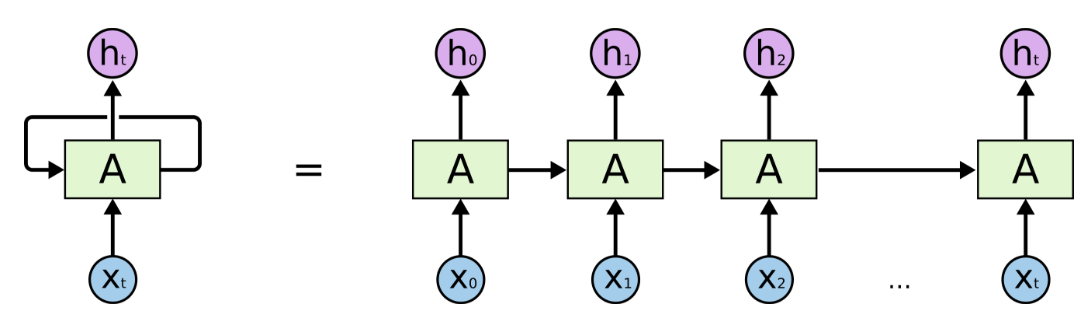
\includegraphics[width=\columnwidth]{images/unfold-rnn.png}
	\caption{An Unrolled Recurrent Neural Network 
	\cite{olah-blog-lstm}}\label{fg:unroll-rnn}
\end{figure}

In previous example, the network is one-directional, i.e. the state at time $t$ 
captures only information from the past, $t-1$, $t-2$,... However, sometimes 
use a bidirectional RNN to allow the current state depends on both previous 
and post information. In particular: ``using bidirectional will run inputs in two 
ways, one from past to future and one from future to past and what differs 
this approach from unidirectional is that in the RNN that runs backwards you 
preserve information from the future and using the two hidden states 
combined you are able in any point in time to preserve information from both 
past and future. Because of their ability to approach a unit from both the 
directions, they tend to understand context better'' 
\cite{aneesh-joshi-LSTM-POS-Tagger}. This could be illustrated in Figure 
\ref{fg:bi-rnn}, where $h^{(t)}$ are states moving forward through time and 
$g^{(t)}$ are states moving backward. The output at each time point is 
depending on both states. 
\begin{figure}[!ht]
	\centering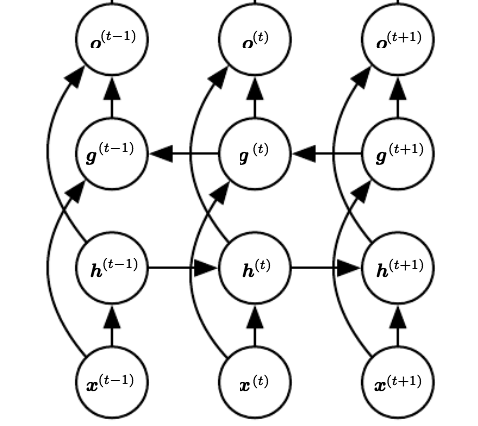
\includegraphics[width=0.7\columnwidth]{images/bi-rnn.png}
	\caption{Bidirectional Recurrent Neural Network 
		\cite{Goodfellow-et-al-2016}}\label{fg:bi-rnn}
\end{figure}

For the Part-of-speech tagging in Section \ref{s:LSTM}, a special RNN is 
used: Long Short-Term Memory Recurrent Neural Network. The details will be 
discussed in that section. 


\section{Warm-up: Word Embeddings and Word2vec}
\label{s:w2v}
This section talks about word embeddings, ``which is the collective name for 
a set of language modeling and feature learning techniques in natural 
language processing (NLP) where words or phrases from the vocabulary are 
mapped to vectors of real numbers. Conceptually it involves a mathematical 
embedding from a space with one dimension per word to a continuous vector 
space with a much lower dimension'' \cite{wiki-wordembedding}. The 
word2vec is a model used to produce word embeddings. It is interesting in 
two ways. First, word2vec itself is a two-layer neural networks that are 
trained to reconstruct linguistic contexts of words, which can be think of as 
a simple application of feedforward networks. Second, using the resulting 
vectors as features for further NLP tasks is considered better in many cases 
due to less human supervised feature engineering. 

\subsection{Model}
The model of word2vec is a two-layer neural networks with one hidden layer 
and one output layer. Given a specific word in the middle of a sentence (the 
input word), the network is going to predict the probability for every word in 
the vocabulary of being the context word i.e. within a certain window of the 
input word. A typical window size is 5, which means 5 words behind and 5 
words ahead of the input word are considered as the context.

The network is trained by feeding word pairs found in training documents 
that are within the window size. Let us assume that the vocabulary is 10000. 
The structure of the network is illustrated in 
Figure \ref{fg:w2v-structure}. 

\begin{figure}[!ht]
	\centering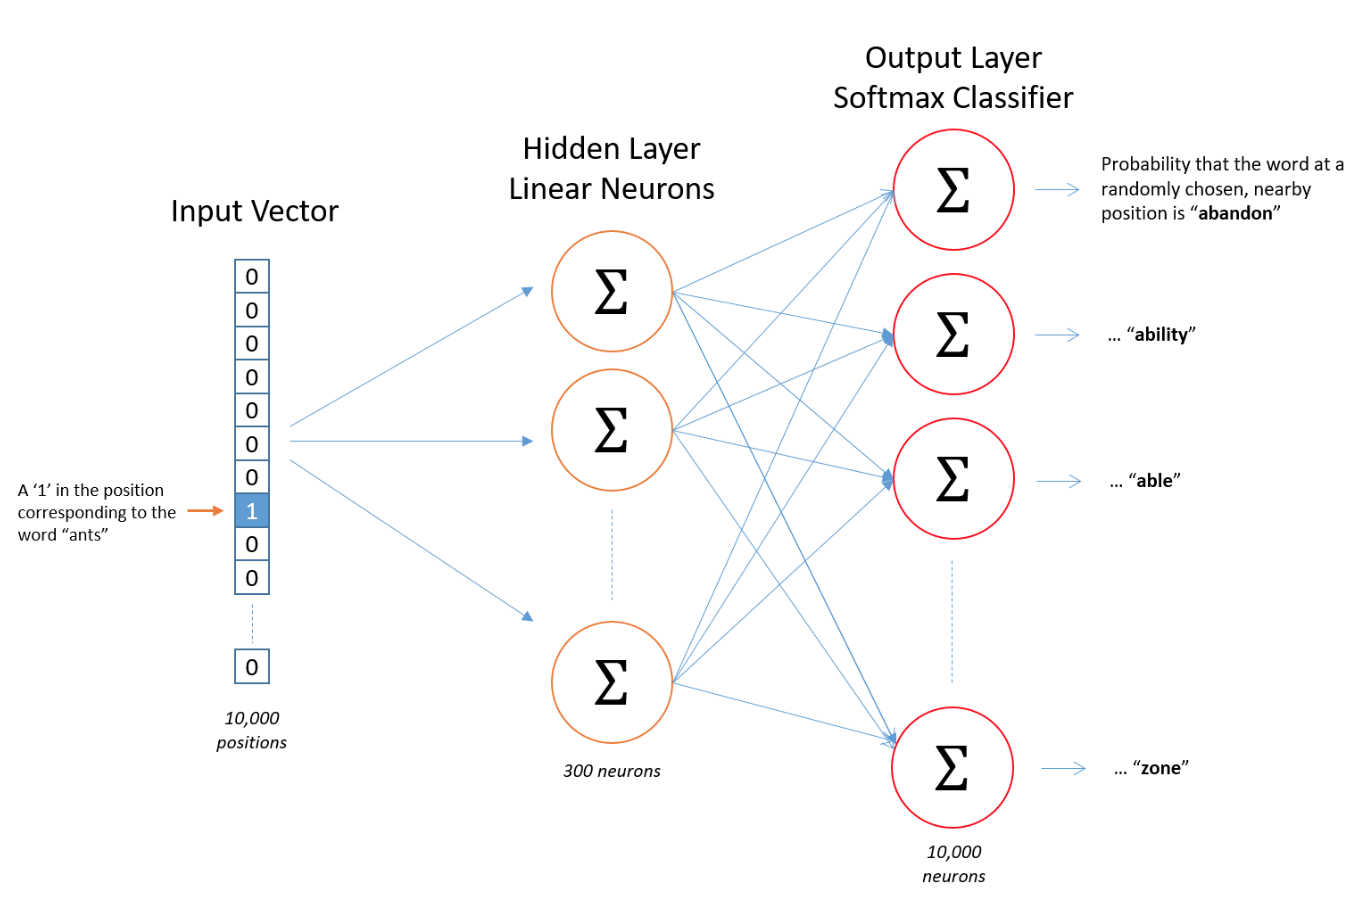
\includegraphics[width=\columnwidth]{images/w2v-structure.png}
	\caption{Structure of Word2vec Network
		\cite{w2v-tutorial}}\label{fg:w2v-structure}
\end{figure}

The input vector is an one-hot vector of length 10000, where only one entry 
is 1 and all others are 0. This vector indicates which input word it represents. 
(Notice there is a one-to-one relationship between the input vector and each 
word in the vocabulary). The hidden layer of size 300, is basically a 
$10000\times 300$ matrix where each role is representing each word in the 
vocabulary in a form of a 300-length real-valued vector. Notice that this 
matrix is what we will save as the ultimate output of our word2vec task, since 
it is the word embeddings for each word. The output of the network is just 
used to tune the numbers in this matrix by comparing with the ground truth. 
(This is why some authors refers this neural network task as a fake task 
\cite{w2v-tutorial}). The output layer which contains the same number of 
neurons as the vocabulary size, is basically a matrix of dimension $300\times 
10000$. By a simple linear algebra calculation we know that taken one input 
vector, the network will output a vector of 10000. After a softmax activation 
function, which normalize these 10000 numbers to a discrete probability 
distribution, we get the probability that each word appear in the context of 
the input word. The loss function could be defined comparing the distance of 
this distribution with the one represented by the ground truth (as provided 
by the training data). 

Training the network involves using techniques such as back propagation to 
minimize the loss function by alternating the weights in the two matrices 
discussed above. 

\subsection{Practical Techniques} 
The word2vec model with a large vocabulary could be very hard to train due 
to the extremely high dimensionality. Mikolov et al discussed several practical 
techniques on top of the basic model above 
\cite{DBLP:journals/corr/MikolovSCCD13}.  There are three innovations in this 
second paper, also discussed by Chris McCormick in his online tutorial 
\cite{w2v-tutorial}, the author will list them below without detailed 
explanation.
\begin{enumerate}
	\item Treating common word pairs or phrases as single “words” in their 
	model.
	\item Subsampling frequent words to decrease the number of training 
	examples.
	\item Modifying the optimization objective with a technique they called 
	“Negative Sampling”, which causes each training sample to update only a 
	small percentage of the model’s weights.
\end{enumerate}

\subsection{Intuition and Implementation}

Using word embeddings such as word2vect representing each word a vector 
provides the syntactic and semantic information about the words which in 
turn can be used for various other tasks. Words which are similar to each 
other are more likely to have similar context therefore the embedding vectors 
are closer in distance. This is the intuition of the model. 

The author did not implement the word2vec model from scratch. Instead, the 
library gensim provides the word2vec model that one could train on his own 
corpora. The word vector for each token can be then provided. The sample 
code is attached here:

 \begin{lstlisting}[language=Python]
import gensim

def train_w2v(sent_list, size=300):
		model = gensim.models.Word2Vec(sent_list, min_count=1,size=size)
		model.delete_temporary_training_data(replace_word_vectors_with_normalized=True)
		return model

def token2vec(token,w2vmodel):
		return w2vmodel.wv[token]
\end{lstlisting}


\section{POS Tagging Using Scikit-learn}
\label{s:pos-sklearn}

This section explains using the library scikit-learn to train a POS tagger with 
hand extracted feature and word embeddings. Different machine learning 
models are applied and the accuracy is around 95\% for hand extracted 
features but relatively low for word embeddings (below 70\%). These could 
be used as a baseline for advanced taggers introduced in Section 
\ref{s:LSTM}. 

\subsection{Data}

The data set I am using for this part is the Treebank tagged sentences 
included in the NLTK (Natural Language Toolkit) package. This is only a small 
fraction (10\%) of the Penn Treebank Corpora, which contains 3914 tagged 
sentences and 100676 tagged tokens. For only learning purpose, I did not try 
to purchase the full Penn Treebank. Another option is the Brown corpora, 
which contains 57340 tagged sentences and a vocabulary of 56057. 

Another reason that I am using the Treebank tagged sentences but not the 
Brown corpus for this part is that due to some unknown limitation of 
scikit-learn (and perhaps my machines), training the neural network on 80\% 
of the Treebank data already causes resource issues. Therefore I can only 
reduce the training proportion to 70\%. In Section\ref{s:LSTM}, I used both 
Treebank and Brown because keras running tensorflow backend has no 
problem even handling Brown Corpus. 

\subsection{Method1: hand crafted features}
As a baseline, I tried to extract some very simple features on each token as 
the input for various models. These features include:
\begin{itemize}
	\item the token itself
	\item if the token is the start of the sentence
	\item if the token is the last of the sentence
	\item if the token is capitalized
	\item if the token has only capital letters
	\item if the token has only lower letters
	\item 3 prefix of the word
	\item 3 suffix of the word
	\item the previous word
	\item the next word
	\item if the word has hyphen
	\item if the word is numeric
	\item if the word has a capitalized word inside (not the first letter)
\end{itemize}


\section[POS Using BLSTM-RNN in Keras]{POS Tagging Using Bidirectional 
Long Short-Term Memory Recurrent Neural Network }
\label{s:LSTM}

\subsection{Deep Learning library: Keras}
\label{s:keras}

\section{Conclusion}
\label{s:conclusion}


\pagebreak
\appendix

\bibliographystyle{abbrv}
\bibliography{report} 

\end{document}
